%%%%%%%%%%%%%%%%%%%%%%%%%%%%%%%%%%%%%%%%%%%%%%%%%%%%%%%%%%%%%%%%%%%%%%%%
%                                                                      %
%     File: Thesis_Background.tex                                      %
%     Tex Master: Thesis.tex                                           %
%                                                                      %
%     Author: Andre C. Marta                                           %
%     Last modified :  2 Jul 2015                                      %
%                                                                      %
%%%%%%%%%%%%%%%%%%%%%%%%%%%%%%%%%%%%%%%%%%%%%%%%%%%%%%%%%%%%%%%%%%%%%%%%

\chapter{Collider experiments}
\label{chapter:exp}

In this chapter we start by providing an overview of the goals and main challenges of modern collider experiments. The definitions of some key quantities that describe an accelerator are introduced and a brief discussion on how they influence the discovery potential of an accelerator is presented. 

In section \ref{section:LHC} we introduce the LHC and in section \ref{section:ATLAS} we describe the ATLAS experiment, including brief discussions on b-tagging, trigger and data acquisition algorithms and systems. In section \ref{section:jet_reco} we introduce the concept of a hadronic jet and describe how these objects are reconstructed in a general collider experiment. Jet properties and substructure observables, as well as jet grooming algorithms, are introduced in sections \ref{section_jet_sub} and \ref{section:jet_groom}, respectively. 

In section \ref{section:future_colliders} we shift the focus to future collider experiments and accelerators and motivate their need. In sections \ref{section:FCC} and \ref{section:FCC_detector} we introduce the hadronic Future Circular Collider (FCC-hh) and describe the baseline detector design, respectively.

Collider experiments are the best tool we have to explore matters' most fundamental structure. 
When we accelerate a particle we increase its momentum. If we take into account the wave particle duality and the De Broglie expression, $\lambda=h/p$, where $\lambda$ is the wavelength and $p$ is the particle's momentum, we can see that a particle with a large $p$ will have a small $\lambda$. The wavelength gives us the dimension scale of the objects we can probe with a given wave. If we want to probe very small particles (subatomic and smaller) we need very small $\lambda$ and therefore very large $p$. Conceptually, this is the basic idea behind modern particle accelerators. 

In practice, charged particles can be accelerated and their trajectories controlled by means of electromagnetic fields. However, this is not without numerous technical challenges. When a charged particle is subject to an acceleration perpendicular to its velocity (which is exactly what happens in circular accelerators) it emits electromagnetic radiation, called synchrotron radiation. The power emitted is proportional to the fourth power of the particle's energy and inversely proportional to the radius squared and to the fourth power of the particle's mass. This radiation limits the maximum energy that can be achieved in electron-positron colliders. In proton-proton colliders, however, the energy is limited by the maximum magnetic field that can be achieved. Therefore, there is also the need for extremely powerful magnets which are usually implemented using technology based in superconductivity. Using superconducting magnets raises another challenge: they can only operate at very low temperatures, close to the absolute zero. In addition, in order to sustain a stable beam it is necessary that the beam pipe has an environment very close to absolute vacuum.   

\section{Experimental aspects}

One of the most important parameters of a particle accelerator is the time integrated luminosity, $\int \mathcal{L}(t) dt$. For a given process with cross section $\sigma$, it determines the number of event that will be produced, $N$:
\begin{equation}
N=\sigma \int \mathcal{L}(t) dt,
\label{eq:n_events}
\end{equation}
where $\mathcal{L}(t)$ is the instantaneous luminosity that is a measure of the number of collisions per bunch crossing.
The instantaneous luminosity is given by:
\begin{equation}
\mathcal{L}=f_{coll}\frac{n_1 n_2}{4\pi\sigma_x \sigma_y},
\label{eq:inst_lumi}
\end{equation}
where $f_{coll}$ is the collision frequency, $n_1$ and $n_2$ are the number of protons in each bunch and $\sigma_x$ and $\sigma_y$ characterize the transverse beam size in the horizontal and vertical directions.

To increase the chances of measuring a rare process, or to increase the statistical significance of the measurement of an already discovered process, we want to increase $N$ as much as possible. To do so we can either increase the integrated luminosity or change the CM energy in order to increase the cross section of the process. 

While the cross sections of most physics processes increase when the CM energy goes from $13$ to $100$ TeV, many BSM models predict new processes, or new contributions to existing processes, whose cross sections increase more rapidly than the SM backgrounds. In addition, by conservation of energy, a larger CM energy implies that particles with larger mass can be created. Based on Eq. \ref{eq:inst_lumi}, we can tune its parameters to obtain the highest possible luminosity. Nonetheless, because we are dealing with charged particles, there is a limit on how close the bunches can be and on how many protons we can pack in a bunch. Moreover, the beam's transverse dimensions cannot be infinitely reduced. A smarter way to increase the number of collisions that an accelerator can produce is to run for a longer time, therefore increasing the integration time in Eq. \ref{eq:n_events}. 

In conclusion, the CM energy and the integrated luminosity are two of the main parameters that drive the discovery potential of an accelerator. 

%Therefore these must be carefully analyzed when planning future accelerators.

%%%%%%%%%%%%%%%%%%%%%%%%%%%%%%%%%%%%%%%%%%%%%%%%%%%%%%%%%%%%%%%%%%%%%%%%
\section{The Large Hadron Collider}
\label{section:LHC}

%IDEAS FOR SECTION
%
%- The LHC: goals and physics programs \\
%- Successes, discoveries \\
%- Upgrades and outlook


The LHC is the world's largest and most powerful particle accelerator. It is housed by the European Organization for Nuclear Research (CERN) which focuses on fundamental particle physics with the goal of probing matter's most elementary structure. Ever since its creation, in 1954, CERN has housed many accelerators and experiments and played a key role in the development of fundamental and applied science.

%(DESCREVER MUITO BREVEMENTE ACELERADORES ANTERIORES? SC, SPS, LEP, ...)

The LHC consists of a $27$-kilometer ring located beneath the Franco-Swiss border, near Geneva. Most of its running time is dedicate to accelerating protons in opposite directions up to a maximum center of mass energy of $\sqrt{s}=13$ TeV and colliding them at the center of the two general purpose experiments, ATLAS (which is described in section \ref{section:ATLAS}) and CMS. The LHCb experiment also records data from proton-proton collisions but it is dedicated to the study of beauty particles. The ALICE experiment is optimized to study heavy-ion collisions at a CM energy of $2.76$ TeV per nucleon.

The acceleration of charged particles at the LHC is based on radio frequency (RF) cavities. These cavities are shaped to sustain a resonant electromagnetic field that oscillates at a frequency of $400$ MHz. During the acceleration stage, charged particles passing through the cavities feel an overall force that propels them forward. When the LHC is running at full energy, a perfectly timed proton with exactly the right energy feels a zero net force when passing the cavities. Protons with a slightly different energies arriving slightly earlier or later are decelerated or accelerated in order to keep the beam sorted in discrete packages with the same energy. These are called bunches. There are $2808$ bunches circulating at the same time, each containing approximately $10^{11}$ protons. The bunches are spaced by $25$ ns. Furthermore, the successful operation of the LHC also relies on superconducting magnets made of Niobium-Titanium filaments chilled to $-271.3\degree$C and on an ultra high vacuum (of the order of $10^{-10}-10^{-11}$ mbar) inside the beam pipes. The magnets are placed along the LHC ring and produce dipole and quadrapole electromagnetic fields. The dipole magnets create a nominal field of $8.3$ T and bend the beam along the tunel. The quadropole magnets focus the beam at the interaction points. The ultra high vacuum greatly reduces the probability that the beam interacts with any particle. It is crucial to keep a stable beam to continuously maintain collisions during long runs.

%In a hadronic accelerator, the maximum reachable energy is usually limited by its circumference and by the magnetic field strength of the bending magnets. The instantaneous luminosity, $\mathcal{L}$, is a measure of the number of events that the accelerator can produce per bunch crossing. It depends on the frequency of the collisions, $f_{coll}$, on the number of particle in each bunch, $n_1$ and $n_2$, and on how focused the beams are when they collide:
%where $\sigma_x$ and $\sigma_y$ characterize the transverse beam size in the horizontal and vertical directions. Based on \ref{eq:inst_lumi}, we can tune its parameters to obtain the highest possible luminosity. Nonetheless, because we are dealing with charged particles, there is a limit on how close the bunches can be and on how many protons we can pack in a bunch. Moreover, the beam's transversal dimensions cannot be infinitely reduced. A smarter way to increase the number of collisions that a accelerator can produce is to leave running for longer. This does not increase the instantaneous luminosity but it increases the integrated luminosity that is given by $\int \mathcal{L}(t) dt$. 
%By conservation of energy, a larger CM energy implies that particles with larger mass can be created. In addition, while the cross sections of most physics processes increase with the CM energy, many BSM models predict new processes, or new contributions to existing processes, whose cross sections increase more rapidly than the SM backgrounds as a function of the CM energy. When it comes to luminosity, we want it to be as high as possible. More collisions means that we have a higher probability of producing rare processes.  
%As initially described in the letter of intent \cite{ATLAS_letter}, the ATLAS experimental program using proton-proton collisions focuses on the exploration of the Higgs and top quarks sectors in different decay channels, on the measurement of Charge Parity (CP) violation in B mesons decays, on the search for supersymmetry (SUSY), new vector bosons and quark substructure and on the study of gauge boson pair production. 

One of the main research goals of the LHC was to discover the Higgs boson. This was achieved in 2012 when ATLAS and CMS reported the discovery of a particle consistent with the boson predicted by the Higgs mechanism, with a mass of $125$ GeV \cite{higgsDiscoveryATLAS},\cite{higgsDiscoveryCMS}. Ever since, efforts have been directed to measuring its mass, couplings, spin-parity properties with increasing precision using different decay channels and production modes. 

ATLAS and CMS reported the observation (measurement with a significance greater than five sigma) of the Higgs decaying to $b\overline{b}$ \cite{ATLASh2bb_discovery, CMSh2bb_discovery}. The searches targeted the $VH$ production mode. It offers the best sensitivity to the $hb\bar{b}$ Yukawa coupling because requiring a vector boson helps reduce the SM backgrounds, namely the ones from QCD interactions. The observation of $h\rightarrow b\overline{b}$ means we have now observed most of the Higgs boson's decay modes predicted by the SM. CMS reported the first observation of the Higgs boson decaying to a pair of tau leptons \cite{CMSh2tautau}. In addition, the observation of Higgs boson production in association with a $t\overline{t}$ pair was very recently reported by both collaborations \cite{CMStth, ATLAStth}. Moreover, precision measurements of the masses of the Higgs \cite{ATLAShMass,hMass} and $W$ \cite{ATLASwMass} bosons and of the top quark \cite{ATLAStopMass, CMStopMass} were also performed. 
So far, no conclusive signs of new physics were seen at the LHC.
%Other LHC results:\\
%- h to bb (evidence) ATLAS+CMS \\
%- h to tau tau (discovery) CMS \\
%- ttH (discovery) ATLAS+CMS \\
%- t production in proton-lead collisions (CMS) ? \\
%- Precision measurements: top, W and Higgs mass \\
%- LHCb results: lepton universality, 5 new particles, ... ? \\
%- No conclusive signs of new physics; constrain models

Future prospects for the LHC include its upgrade to the High Luminosity-LHC (HL-LHC) after
the scheduled long shutdown of 2024-2026. This upgrade will increase the size of the dataset to $3000~\text{fb}^{-1}$ over the course of ten years \cite{High-Luminosity}. 
During the shutdown, the ATLAS detector will be upgraded. 

%MAIN UPGRADES (namely, refer TileCal high granularity upgrade ?)

%HL-LHC physics programme:\\
%- Higgs precision measurements (properties and couplings) \\
%- Higgs rare processes: h to mu mu, h to J/Psi \\
%- Higgs self couplings \\
%- BSM searches: SUSY, 2HDM, ...\\

In the Higgs sector, the high value of the integrated luminosity will improve the statistical precision of already measured channels and the discovery potential of rare processes \cite{HL_LHC}.

\subsection{The ATLAS detector}
\label{section:ATLAS}

The ATLAS detector has a cylindrical geometry and a multi layered structure. Its dimensions are $25$ meters in height (diameter) and $44$ meters in length and it weights approximately $7000$ tonnes. In the following paragraphs we describe the detector's layers and their functionalities. A schematic representation of the detector as well as the appropriate coordinate system can be found in figure \ref{fig:ATLAS_detector}.

A combination of cartesian and cylindrical coordinates is used to describe the detector. In both cases, the origin is defined to coincide with the interaction point. The Cartesian system is right-handed and the z axis is defined to be the direction of the beam. The x-axis points from the interaction point to the center of the LHC ring and the y-axis points upwards. The azimuthal angle, $\phi$, is measured around the beam axis and the polar angle, $\theta$, from the beam line. The pseudorapidity is defined as $\eta=-\ln \tan(\theta/2)$. Another commonly used quantity is the rapidity, $y$, defined as a function of a particle's energy, $E$, and longitudinal momentum, $p_L$: $y=\frac{1}{2}\ln \left(\frac{E+p_L}{E-p_L}\right)$. In the limit where a particle's mass is negligible with respect to its momentum the pseudorapidity converges to the definition of rapidity. In addition, the angular distance between two points, $\Delta R$, is defined as $\Delta R=\sqrt{(\Delta \phi)^2+(\Delta \eta)^2}$, where rapidity can also be used instead of the pseudorapidity. 

The detector consists of an inner detector (ID) or tracker, electromagnetic (EM) and hadronic calorimeters and a muon spectrometer (MS).
The magnet configuration consists of a thin superconducting solenoid that surrounds the ID cavity and three superconducting toroids (one barrel and two end-caps) arranged with an eight-fold azimuthal symmetry around the calorimeters.

The ID covers the pseudorapidity range $|\eta|<2.5$ and it makes up the innermost layer of the detector. It consists of silicon pixel, silicon micro-strip, and straw tube transition radiation tracking detectors. It is contained in a solenoid magnet with a central field of $2$ T. The tracker provides precision measurements of the positions and momenta of charged particles. As a charged particle transverses the several layers of the ID it ionizes the medium creating electrical signals that can be read out. These individual electrical signals are then combined to reconstruct the trajectory of the particle. 

Lead/Liquid-Argon (LAr) sampling electromagnetic (EM) calorimeters cover the pseudorapidity range $|\eta|<3.2$. The EM calorimeter has an accordion like structure with layers of showering material (lead) interleaved with layers of active material (liquid argon). These calorimeters provide measurements of the energy of electrons and photons. The interaction of these particles with the lead layers induces the production of an EM shower whose energy  is measured in the liquid argon layers. The granularity of the EM calorimeter strongly depends on the longitudinal layer and on the pseudorapidity region. 

The hadronic calorimetry in the pseudorapidity range $|\eta|<1.7$ is provided by a scintillator-tile calorimeter (TileCal) which is divided in a central barrel and two smaller end-cap barrels, one on each side of the central barrel. The active components are scintillator tiles made of polystyrene that are interleaved with steel plates as the passive material. The scintillation light emitted by the tiles when an ionising particle crosses the calorimeter is collected on both ends of the tiles by wavelength-shifting optical fibers. The light signal emitted is proportional to the particle's energy. The TileCal is composed of several cells with transverse segmentation $\Delta\eta\times\Delta\phi=0.1\times0.1$ \footnote{The TileCal is composed of three longitudinal layers. Only the first two have a segmentation equal to $0.1\times 0.1$. In the third layer the segmentation is $0.2\times 0.1$. However, most of the energy of hadronic showers is deposited in the first layers and therefore this detail is not very relevant for this work.} \cite{TileCalTech}. 

For $|\eta|>1.5$ LAr calorimeters extend the pseudorapidity range to $|\eta|=4.9$. The LAr calorimeter is divided in end-cap and forward. These cover the pseudorapidity ranges $1.5<|\eta|<3.2$ and $3.2<|\eta|<4.9$, respectively. The active material is liquid-argon and the absorbers are copper and tungsten for the end-cap and forward calorimeters, respectively. In the end-cap LAr calorimeters the segmentation is $\Delta\eta\times\Delta\phi= 0.1\times0.1$ for $1.5<|\eta|<2.5$ and $0.2\times0.2$ for $2.5<|\eta|<3.2$. In the forward LAr calorimeter the segmentation is $\Delta\eta\times\Delta\phi= 0.2\times0.2$. 

The granularity of the ATLAS hadronic calorimeters is summarized in table \ref{table:ATLAS_HCAL}.

\renewcommand{\arraystretch}{1.2}

\begin{table}
	\centering
	\caption{ATLAS tile and liquid argon hadronic calorimeters: summary of the pseudorapidity coverages and transversal segmentation (granularity).}
	\begin{tabular}{llll}
		\toprule 
		\textbf{TileCal} & \textbf{Barrel} & \textbf{Extended barrel} &\\
		\midrule
		\rowcolor{black!7}Coverage & $|\eta|<1.0$ & $0.8<|\eta|<1.7$  & \\
		Granularity & $0.1\times 0.1$ & $0.1\times 0.1$ & \\
		\midrule \midrule
		\textbf{LAr calorimeter} & \textbf{End-cap} & \textbf{Forward} &\\
		\midrule
		\rowcolor{black!7}Coverage & $1.5<|\eta|<3.2$ & $3.2<|\eta|<4.9$  &  \\
		\multirow{2}{*}{Granularity} & $0.1\times 0.1 ~\text{for}~ 1.5<|\eta|<2.5$ & \multirow{2}{*}{$0.2\times 0.2$} & \\
		& $0.2\times 0.2 ~\text{for}~ 2.5<|\eta|<3.2$ & & \\
		\bottomrule
	\end{tabular}
	\label{table:ATLAS_HCAL}
\end{table}

The hadronic calorimeters provide measurements of the energy of hadrons, jets; these allow the estimation of the missing transverse energy $\left(E_T^{miss}\right)$. Approximately one third of the energy of jets is deposited in this layer. In the TileCal, the jet energy resolution is given by $\sigma/E\sim 50\%/\sqrt{E}+3\%$ \cite{TileCalTech},
where the first term is the stochastic term that derives from sampling fluctuations and follows a Poisson distribution and the second term is a constant that depends on the characteristics of the calorimeter. For the LAr calorimeter, the jet energy resolution is given by $\sigma/E\sim 60\%/\sqrt{E}+2\%$ \cite{ATLAS_LAr_TDR}.

The MS is the outermost layer of the detector and it is dedicated to detecting muons that travel through the previous layers almost without interacting. This layer provides measurements of the muons transverse momenta. It is composed of Monitored Drift Tubes (MDT) and Cathode Strip Chambers (CSC) that provide high precision measurements of the muons' momentum in the pseudorapidity range $|\eta|<2.7$ and of Resistive Plate Chambers (RPC) and Thin Gap Chambers (TGC) dedicated to triggering purposes for $|\eta|<2.4$.

\begin{figure}
	\centering
	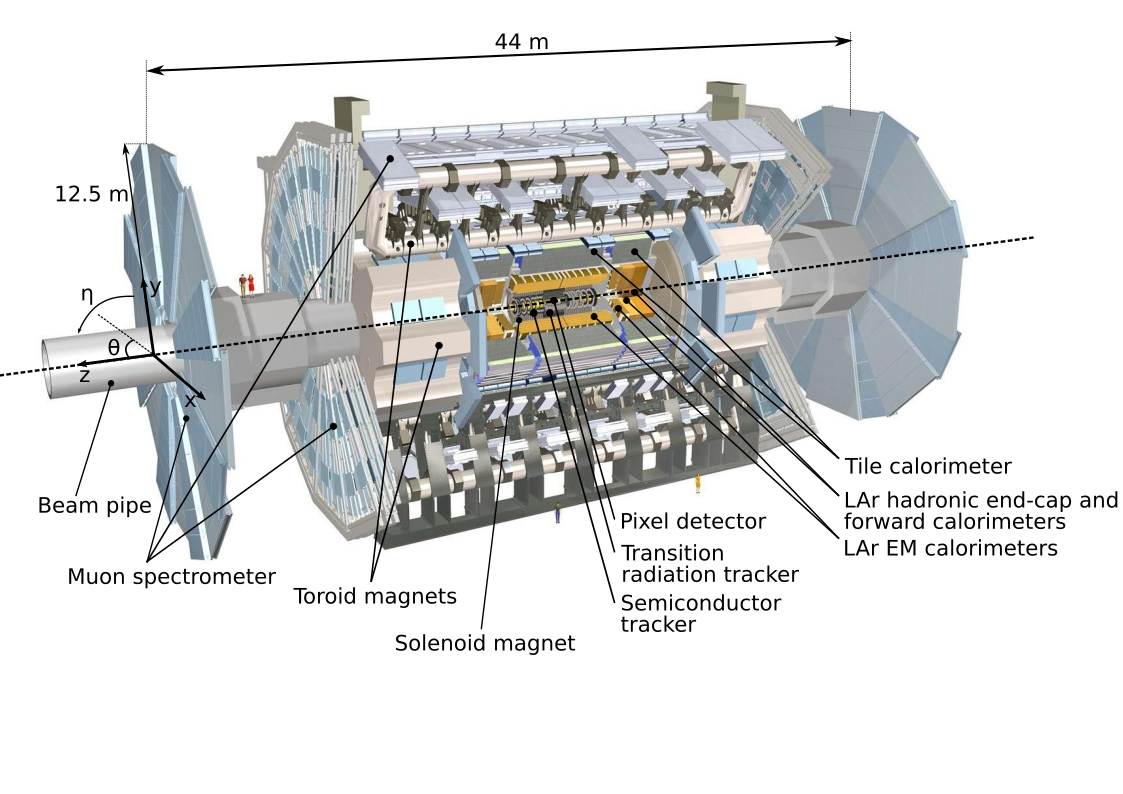
\includegraphics[trim={0cm 3.5cm 0cm 0},clip,width=\textwidth]{./Figures/ATLASsvg3.png}
	\caption{ATLAS detector.}
	\label{fig:ATLAS_detector}
\end{figure} 

\subsubsection{b-Tagging}

Each collision produces a large number of hadronic jets (we refer to section \ref{section:jet_reco} for a detailed description of jets and how they are reconstructed). For this work, jets initiated by a b quark (b jets) are particularly important: we are looking for a Higgs pair decaying to four b quarks which leads to an experimental signature that consists of four b jets. b-Tagging algorithms determine, with a given probability, if a jet was originated by a b quark. 

When a b quark is produced it hadronizes almost instantly, producing a B hadron. B hadrons have a lifetime of $\sim$ 1 ps and can be highly relativistic meaning that they can travel a few millimeters to a few centimeters inside the inner detector before decaying. When they decay there is often a reconstructible secondary vertex that is slightly displaced from the primary vertex where the b-quark was produced. The existence of a secondary vertex is used by b-tagging algorithms to identify, or tag, a jet as coming from a b-quark. It is important to note that a complete b-tagging algorithm relies on the reconstruction of a secondary vertex which can only be done using the information form the inner detector. This implies that, in ATLAS, we can only b-tag jets that are produced in the region $|\eta|<2.5$.

In ATLAS, b-tagging algorithms are applied to the sub-set of tracks that are associated with a given jet. The matching between tracks and calorimeter-based jets is performed using the ghost association technique \cite{GhostAssociation}\footnote{This procedure works by introducing ghost versions of the measured tracks that have the same direction but infinitesimally small $p_T$ such that they do not modify the properties of the calorimeter jets. The jets are then reclustered and a track is considered to be associated with a given jet if its ghost version is contained in the jet after reclustering.}. The identification of b-jets in ATLAS is based on distinct strategies encoded on three b-tagging algorithms: impact parameter-based algorithms, an inclusive secondary vertex reconstruction algorithm and  a decay chain multi-vertex reconstruction algorithm. The output of these algorithms are combined in a multivariate discriminant based on a Boosted Decision Tree (BDT) which provides the best discrimination between the different jet flavors \cite{btagATLAS}.

The impact parameter-based algorithms \cite{ATLASbtag}, IP2D and IP3D, use as discriminant variables the transverse impact parameter significance and the transverse and longitudinal impact parameter significance, respectively. The secondary vertex finding algorithm \cite{ATLASbtag}, SV, explicitly reconstructs a displaced secondary vertex inside the jet by trying to find pairs of tracks with a common origin. The decay chain multi-vertex reconstruction algorithm \cite{ATLASbtag1}, JetFitter, tries to reconstruct the full b-hadron decay chain. This approach allows to resolve b- and c-hadrons vertices even if there are not two tracks associated with them.

\subsubsection{Trigger and data acquisition}

The LHC delivers approximately 1000 million proton-proton collisions per second, which corresponds to an event rate of 1 GHz. On the one hand, only a small fraction of these events result in interesting physics processes. On the other hand, the detector does not have enough storage or read out capabilities to record all the collisions. The triggering and data acquisition systems are responsible for selecting a manageable rate of events for permanent storage and further analysis. 

The trigger is responsible for selecting events with interesting experimental signatures. The trigger system in Run-2 consists of a hardware-based first  level  trigger (Level-1) and a software-based high level trigger (HLT). The Level-1 trigger takes as input  coarse  granularity calorimeter and muon detector information and reduces the event rate to 100 kHz. The HLT uses full granularity detector information and reduces the rate to approximately 1 kHz \cite{run2trigger}.    

%[USE ANOTHER EX?] Take, as an example, the inclusive cross section for the production of jets which is of the order of $10^6$ fb. If we consider a luminosity of $0.8~\text{fb}^{-1}$ per day, this corresponds to a rate of approximately 200 Hz, just for the production of jets. Note that this value is the same as the maximum allowed rate for all physics processes after all the triggers. Therefore, it is clear that we cannot simply take all the jet events. We need to place tight cuts that allow us to reduce this rate to an acceptable (within the available quotas) rate. This is of particular importance for processes with very large cross sections such as QCD multijet production.

%\begin{figure}
%	\centering
%	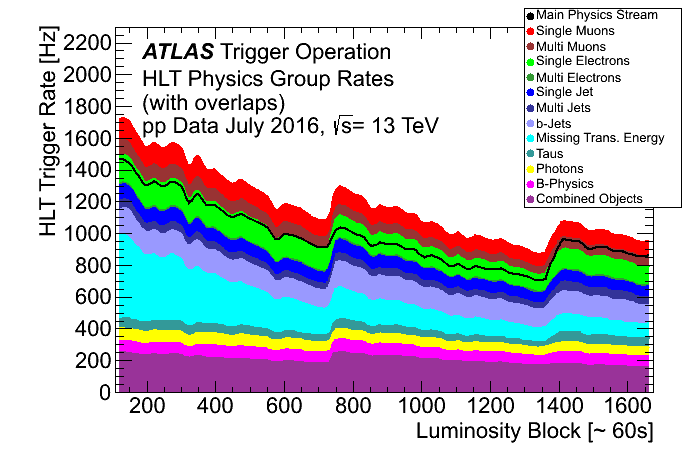
\includegraphics[width=0.7\linewidth]{./Figures/HLT.png}
%	\label{fig:HLT}
%	\caption{oi}
%\end{figure}

%\begin{figure}[!tbp]
%	\centering
%	\begin{minipage}[b]{0.4\textwidth}
%		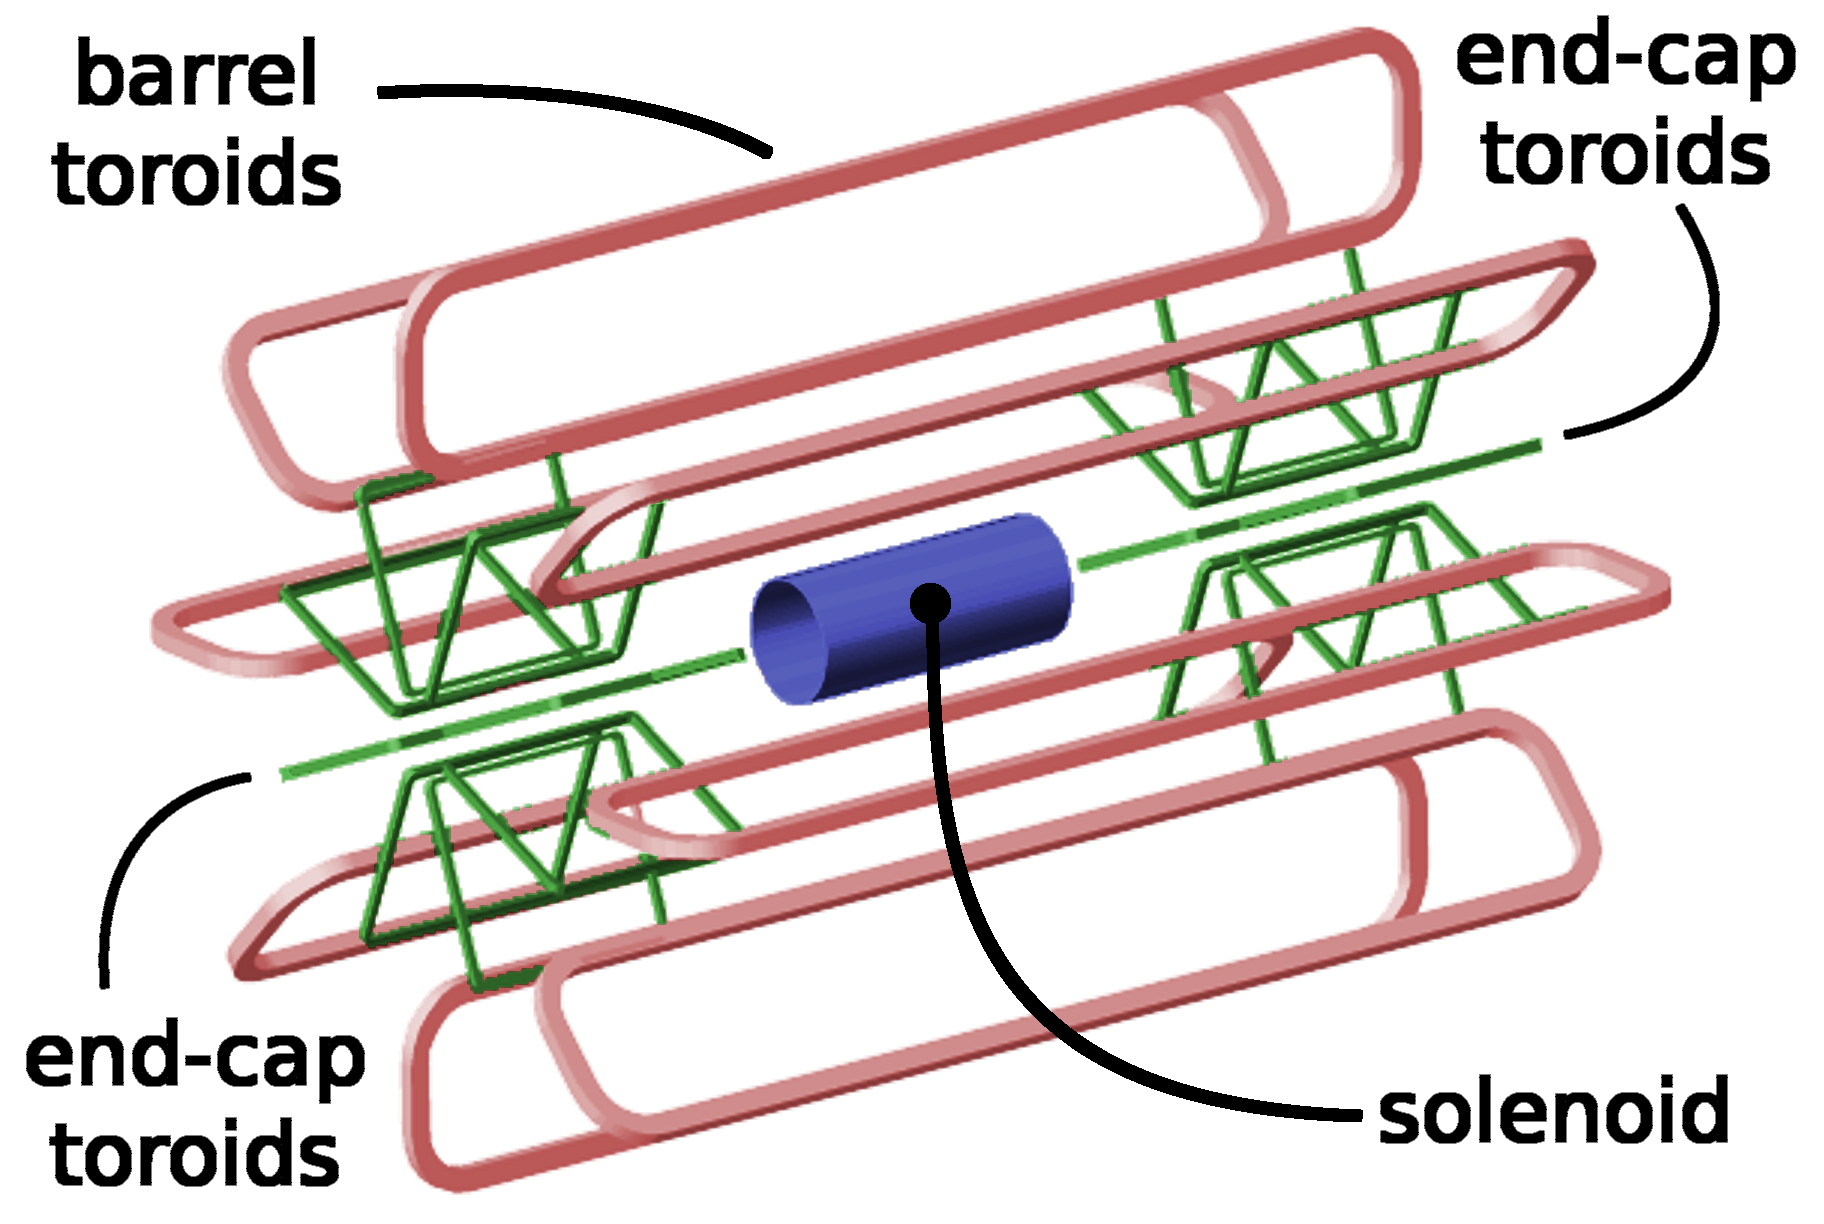
\includegraphics[width=\textwidth]{./Figures/magnetSystems.png}ing system 
%		\caption{Flower one.}
%	\end{minipage}
%	\hfill
%	\begin{minipage}[b]{0.4\textwidth}
%		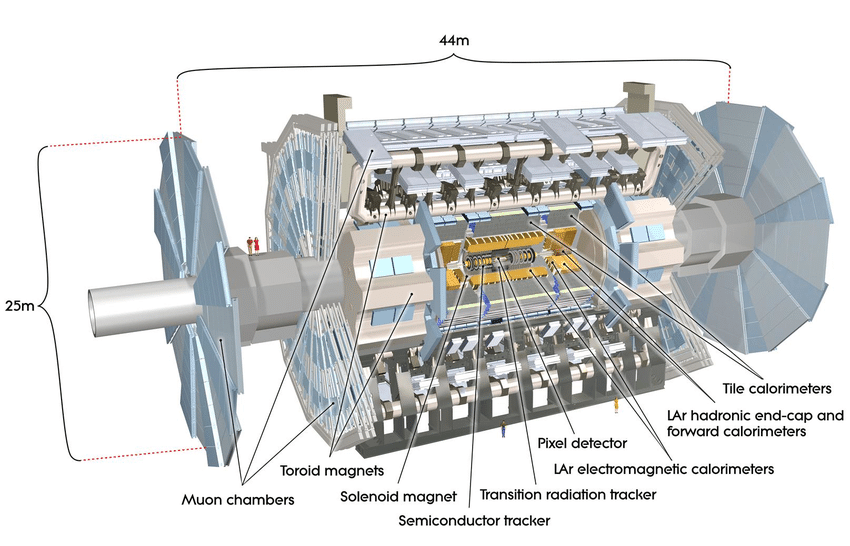
\includegraphics[width=\textwidth]{./Figures/ATLAS.png}
%		\caption{Flower two.}
%	\end{minipage}
%\end{figure}

%\begin{figure}
%	\centering
%	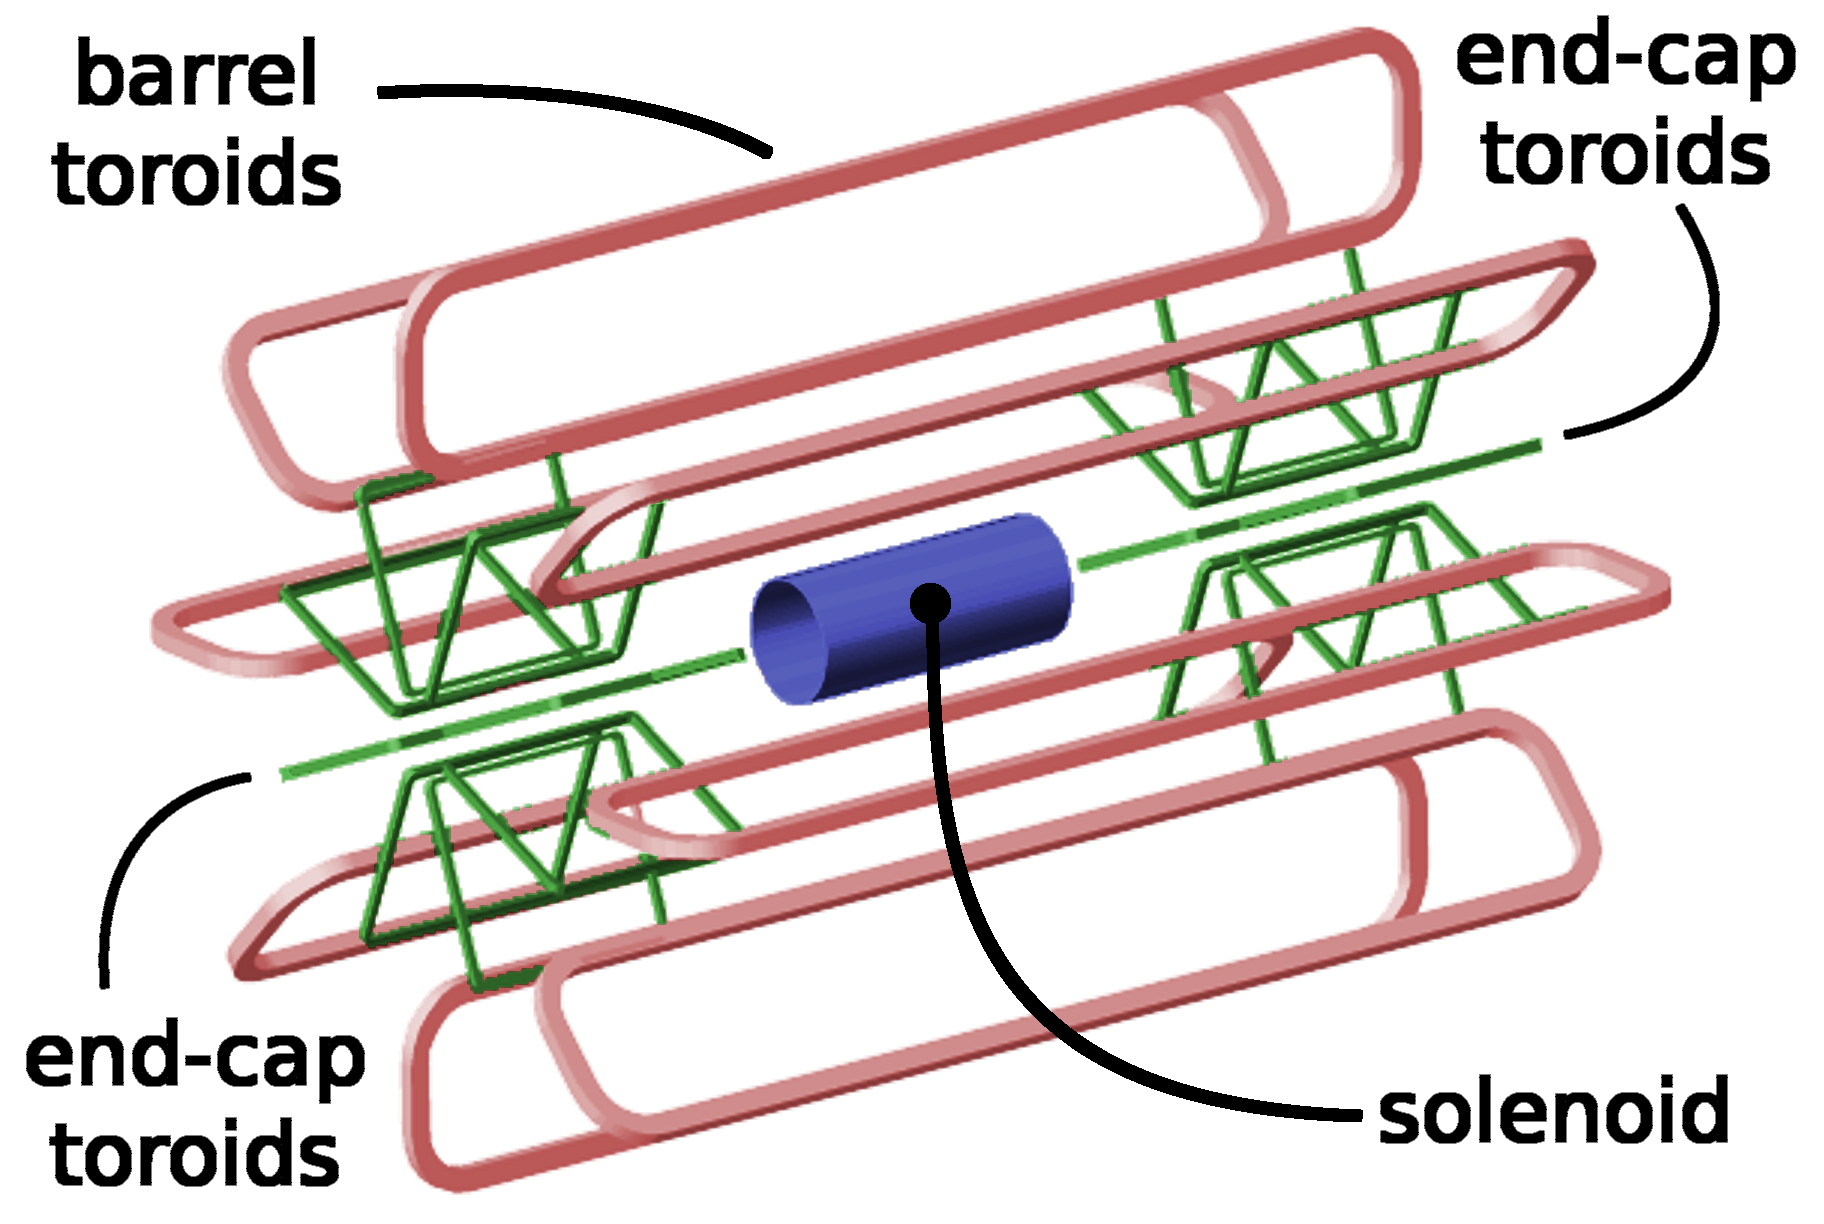
\includegraphics[width=0.5\textwidth]{./Figures/magnetSystems.png}
%	\caption{ATLAS detector magnet configuration.}
%	\label{fig:ATLAS_magnet}
%\end{figure}     

%%%%%%%%%%%%%%%%%%%%%%%%%%%%%%%%%%%%%%%%%%%%%%%%%%%%%%%%%%%%%%%%%%%%%%%%

\section{Jet reconstruction}
\label{section:jet_reco}

A jet is a collimated spray of hadrons that is interpreted as coming from a single initial parton such that approximately retains information about its physical properties, namely 3-momentum, mass and charge. The existence of such objects is a direct consequence of the confinement property of QCD. Quarks and gluons, the fundamental degrees of freedom of QCD, are not asymptotically free. They are confined inside hadrons. Therefore, when one of these particles is produced it undergoes showering and hadronization processes that lead to the formation of hadrons.

At a particle detector we are interested in reconstructing jets. These are the objects that are used in the physics analysis. Working with jets instead of hadrons is an advantage because it greatly reduces the number of objects we need to analyze per event. In addition, they work as a \textit{proxy} for the fundamental partons produced in the event.

Jets are obtained through jet finding algorithms. These are clustering algorithms that group together experimental quantities (energy deposits in the calorimeters, tracks or particle flow objects) using a sequential recombination scheme. If the jets are reconstructed using only the information from the energy clusters in the calorimeter they are called calorimeter or tower jets. Jets can also be reconstructed using particle flow objects that combine information from the tracking system and from the calorimeters. These jets are referred to as particle flow or energy flow jets (eflow in short).

A crucial property of jet finding algorithms is that they should be infrared and collinear safe, meaning that the outcome of the algorithm (namely the number of jets and their properties) should not be significantly
modified by the emission of soft radiation or by a collinear splitting.

The most widely used jet finding algorithms are the $k_T$ \cite{kt}, the Cambridge/Aachen (C/A) \cite{CA} and the anti-$k_T$ \cite{anti-kt}. They are based on measurements of the quantity:

\begin{equation}
d_{ij}=\min(k_{Ti}^{2p},k_{Tj}^{2p})\frac{\Delta_{ij}^2}{R^2}, \qquad
d_{iB}=k_{Ti}^{2p},
\end{equation}
referred to as a distance between entities $i$ and $j$ with $d_{iB}$ being the distance between entity $i$ and the beam ($B$). $\Delta_{ij}^2=(y_i-y_j)^2+(\phi_i-\phi_j)^2$ and $k_{Ti}$, $y_i$ and $\phi_i$ are the transverse momentum, rapidity and azimuth of entity $i$. Here, $k_{T}$ stands for the transverse momentum. For $p=1,0,-1$ we get the $k_T$, C/A and anti-$k_T$ algorithms, respectively.

The clustering algorithm starts by computing all $d_{ij}$ and $d_{iB}$ distances. If the smallest distance is a $d_{ij}$, the four momenta of particle $i$ and $j$ are summed and the distances are updated. If the smallest distance is a $d_{iB}$, particle $i$ is removed and called a jet. This procedure is iterated until all particles are clustered in jets.

It is worth discussing further the anti-$k_T$ algorithm since it is the default algorithm used in most analyses, including this one. In this algorithm, the $\Delta_{ij}$ distance between constituents $i$ and $j$ is weighted by the inverse of the transverse momentum of the constituent with a largest $k_T$. This feature implies that particles with larger momenta will have a smaller $d_{ij}$ distance and therefore will be clustered first. This prevents soft particles from being clustered among themselves before clustering the hardest particles.

In ATLAS, the transverse and longitudinal segmentation of the calorimeters allow for a three dimensional reconstruction of particle showers which is based in a topological clustering algorithm. Topo-clusters of calorimeters cells are seeded by cells whose absolute energy exceeds the electronic and pile-up noise by four standard deviations. The topo-clusters are then expanded by adding all adjacent cells with absolute energy two standard deviations above noise. Finally, all cells neighbouring the previous set are also added. After energy calibration, the topo-clusters are fed as input to a jet finding algorithm.  

\subsubsection{Boosted kinematic regime}

With the increase of the CM energy of particle colliders the production of particles with a transverse momentum much larger that their mass became a reality. In this kinematic regime (referred to as boosted due to the high Lorentz boost of the particles) traditional jet reconstruction algorithms, that rely on a one-to-one correspondence between jets and partons, begin to fail \cite{jetsubLHC}. 

Due to the high Lorentz boosts, decay products of heavy resonances get more collimated. The angular separation of the decay products is approximatelly \cite{jetsub}:
\begin{equation}
	\Delta R \sim \frac{2 m}{p_T}
	\label{eq:deltaR}
\end{equation}
where $p_T$ and $m$ are the transverse momentum and mass of the decaying particle. In addition to decaying particles with a larger $p_T$, another event topology that can produce highly collimated particles is the decay of a particle with a very large mass. This scenario is of particular interest for new physics searches because BSM models often predict the existence of heavy particles. 

Take, as an example, the decay of a Higgs boson to two b quarks. Considering that the $p_T$ of the Higgs is approximately $200$ GeV (which is a reasonable and commonly used value in boosted Higgs bosons searches) we get $\Delta R \sim 1$. For resolved jets, the default jet radius parameter used in ATLAS is $0.4$. We see that for a $p_T \sim 200$ GeV the angular separation between the decay products of a Higgs boson is already similar to the default jet diameter, which can jeopardize the ability to resolve the individual decay products.

%There is a limit after which it is no longer possible to reconstruct both decay products as individual jets because the $\Delta R$ between the decay products has a value that is very close to the jet's diameter such that we start to have an overlap between the two jets (?).

A possible workaround is to use a single jet with a larger $R$ parameter to reconstruct both decay products. The problem with doing so is that we no longer have information about each individual decay product which means we are loosing some information about the event. We cannot, for example, compute angular variables between the decay products. This led to the development of techniques and observables that allow for the exploration of the intrinsic structure (or substructure) of these large-$R$ jets. Some of these techniques are introduced and discussed in the following section.  

\subsection{Jet properties and substructure observables}
\label{section_jet_sub}

%TO INCLUDE (it will depend on the ones that are most important to the analysis):\\
%- tau\_N \\
%- energy correlation functions and ratios \\
%- Fox Wolfram\\
%- ...\\
%- Jet mass definition!\\

%Perhaps the most used jet observable is the invariant mass, $M$, that is  calculated from the energies and momenta of its constituents as follows:
%\begin{equation}
%	M=\left(\sum_{i}E_i\right)^2-\left(\sum_{i}\vec{p}_i\right)^2
%\end{equation}
%where $E_i$ and $\vec{p}_i$ are the energy and three-momentum of the $i^{th}$ constituent. If we are dealing with large-R jets, the mass can be used as an approximation of the resonances's mass. 

In general, jet substructure variables aim to quantify the existence of energy clusters  insider a jet. Each cluster is interpreted as corresponding to an individual jet. These are called subjets because they are contained inside the large-$R$ jet that was reconstructed. Once they are identified, the subjets can be handled and used for the analysis like normal jets. However, a lot of the substructure techniques do not focus on reconstructing the subjets but rather on determining whether or not they exist, how many they are and how are they distributed inside the large-$R$ jet. 

Heavy resonances decaying to two(three) particles will produce large-$R$ jets that are consistent with the existence of two(three) energy clusters. Examples of such topologies are the Higgs boson and top quark decays: the Higgs boson always decays to pairs of particles (leptons, quarks or bosons) and the top quark decays, with a probability close to $100\%$, to a $b$ quark and a $W$ boson that then decays to a pair of leptons or quarks. These topologies are usually referred to as two or three prong. In contrast, jets initiated by a gluon or quark splitting are not expected to have a meaningful substructure. The energy is expected to be concentrated around the jet axis following an isotropic distribution and to become less dense as we approach the jet's border. This is the signature of a one-prong topology. The previous discussion is valid at LO and captures the generic features of jets that are targeted by jet substructure techniques. Nonetheless, other effects may come into play. Take, for example, a highly virtual gluon with a high $p_T$. If it splits into two quarks the resulting jet may have two subjets and thus mimic the topology of a heavy resonance decay.

The N-subjetiness variable \cite{Nsubjetiness}, $\tau_N$, may be used to identify jets compatible with N subjets. It is given by 
\begin{equation}
	\tau_N = \frac{1}{d_0}\sum_{k}p_T^k \min(\Delta R_1^k,...,\Delta R_N^k), \qquad d_0=\sum_{k}p_T^k R_0
\end{equation}
where the index $k$ runs over all particles in a jet, the indexes $1$ to $N$ identify the number of axis inside the jet and $R_0$ is the radius of the jet. This variable will have a small value if the particles with the highest $p_T$ (the ones we are most interested in) are clustered around the axis (because $\Delta R$ will be small) and will have a larger value otherwise. A jet with small $\tau_N$ is considered to be consistent with having $N$ or fewer subjets because all its constituents are aligned with the axis.

We usually use ratios of $\tau_N$ variables ($\tau_{MN}=\tau_M/\tau_N$). Of particular interest for this work are the $\tau_{21}$, $\tau_{31}$ and $\tau_{32}$ ratios. These observables can take values between zero and one. For $\tau_{21}$, for example, a small value (close to zero) indicates that the jet is more compatible with two subjets than with one and therefore it can help discriminate between two-prong and one-prong jets. The same applies to every other ratio. 

The Fox-Wolfram moments, $H_l$, can be used to identify jets that have a structure of two back-to-back subjets in their rest frames \cite{FW2}. They are given by:
\begin{equation}
H_l = \sum_{i,j}\frac{|\vec{p}_i||\vec{p}_j|}{E^2}P_l(\cos(\theta_{ij}))
\end{equation}  
where $\theta_{ij}$ is the opening angle between energy clusters $i$ and $j$ with respect to the interaction point, $E$ is the total energy of the clusters in the jet rest frame and $P_l(x)$ are the Legendre polynomials. For a jet that has a structure of two back-to-back subjets in its rest frame, $H_1 = 0$, $H_l \sim 1$ for even l, and $H_l \sim 0$ for odd l. This is what we expect for jets coming from the decay of a boosted resonance. In this work we make use of $H_2$.

In addition to jet substructure observables, more standard variables, from which we highlight the jet mass, can also be used to discriminate between jets coming from QCD background and jets resulting from heavy resonance decays. In the latter, the jet's invariant mass should roughly correspond to the mass of the resonance. The invariant mass of a jet, $M$, is  calculated from the energies and momenta of its constituents as follows:
\begin{equation}
	M^2=\left(\sum_{i}E_i\right)^2-\left(\sum_{i}\vec{p}_i\right)^2
\end{equation}
where $E_i$ and $\vec{p}_i$ are the energy and three-momentum of the $i^{th}$ constituent. However, the mass resolution is not expected to be very good for large-R jets because of all the extra QCD radiation that may be caught inside the jet. A possible workaround is the use of jet grooming algorithms which we describe in the following section.

\subsection{Jet grooming algorithms}
\label{section:jet_groom}

The main goal of jet grooming algorithms is to remove contamination of softer jet constituents from pileup or underlying event and to leave behind the hard substructure. The main advantage of such algorithms is that they improve the mass resolution of jets. These features are of particular interest in high luminosity environments such as the HL-LHC and future high energy colliders. 

There are three main jet grooming algorithms: trimming, pruning and mass drop filtering. In this work we do not use pruning or trimming, although these techniques might be worth exploring in future, more comprehensive, studies. In particular, they can be useful to help reject pileup contributions. The mass drop filtering procedure isolates relatively symmetric subjets within a jet, each with a significantly smaller mass than the original jet \cite{jetsub}. This technique was developed and optimized using C/A jets for the search of Higgs decaying to $b\overline{b}$ pairs \cite{BDRS}. It works as follows:
\begin{itemize}
	\item The last step of the C/A clustering is undone such that the jet is split in two subjets, $j_1$ and $j_2$ with $m_{j_1}>m_{j_2}$. We require that there is a significant difference between the mass of the original jet, $m_{\text{jet}}$, and $m_{j_1}$: $m_{j_1}/m_{\text{jet}} < \mu_{\text{frac}}$, where $\mu_{\text{frac}}$ is a parameter of the algorithm. In addition the splitting is required to be relatively symmetric:
	\begin{equation}
		\frac{\min[(p_T^{j_1})^2,(p_T^{j_2})^2]}{(m_{\text{jet}})^2} \times \Delta R_{j_1,j_2}^2 > y_{\text{cut}}
	\end{equation}
	where $y_{\text{cut}}$ is a parameter that defines the energy sharing between the subjets. It is usually taken to be $\sim 0.09$. If these two criteria are not met the jet is discarded.
	
	\item The subjets are clustered with the C/A algorithm with radius parameter $R_{\text{filt}}=\min[0.3,\Delta R_{j_1,j_2}/2]$. All jet's constituents that are outside of the three hardest subjets are discarded and we obtained the filtered jet and its subjets.
\end{itemize}

The subjets that are identified within a jet are interpreted as corresponding to the decay products of the particle that produced the original jet. There are usually only two decay products. A third subjet is allowed in order to account for extra QCD radiation.

\section{Future Colliders}
\label{section:future_colliders}

As we already argued in the beginning of this chapter, a larger CM energy is one of the factors driving the discovery potential of an accelerator. As far as we know today, proton-proton colliders are the main, and possibly only, man-made experimental tool available to explore particle physics in the energy range on tens of TeV, in a controlled way. With this in mind, new hadronic colliders with CM energies of the order of tens of TeV have been proposed. The main projects are the hadronic Future Circular Collider (FCC-hh) lad by CERN and the Super Proton-Proton Collider (SPPC) proposed by China. 

In this work we focus on FCC-hh and use the established detector's baseline design as our starting point for this study. In the following section we describe in detail the FCC-hh accelerator and detector.

\subsection{The hadronic Future Circular Collider}
\label{section:FCC}

%IDEAS FOR SECTION
%
%- Center of mass energy \checkmark \\
%- Basic design: circular, circumference, location, ... \checkmark\\
%- CERN FCC study group: creation, mission, main tasks \checkmark \\
%- The role of the hadronic calorimeter \\
%- Basic structure: tracker, calorimeters, muon chambers \checkmark \\
%- Technical specifications: nb. bunches, magnets, ... \checkmark\\
%- Technical dimensions and materials (predictes) of each layer \checkmark\\
%- Focus on hadronic calorimeter: material being studied, resolution, granularity \checkmark\\
%- What processes we want to study at the FCC \\
%- Focus on Higgs pair production \\

CERN's FCC study group was launched as a result of a recommendation made in the  2013 update of the European Strategy for Particle Physics that '\textit{Europe needs to be in a position to propose an ambitious post-LHC accelerator project at CERN by the time of the next Strategy update}'. It investigates the technological challenges and physics opportunities of a future circular collider. The design and infrastructure are driven by a proton-proton collider (FCC-hh) requirements. Electron-positron (FCC-ee) and electron-proton (FCC-eh) colliders are also being analyzed. The main goal of this effort is to deliver a Conceptual Design Report (CDR) by the end of 2018. This document will include a first cost estimate to be submited for the next update of the European Strategy for Particle Physics, foreseen by 2020.

The FCC-hh baseline design consists of a proton-proton circular collider with a maximum CM energy of $100$ TeV housed by a $100$ km tunnel in the area of Geneva. This machine will extend the research program of the LHC (and of the HL-LHC) after these have reached their full discovery potential, by around 2040. In addition, it will allow for the exploration of an entirely new kinematic regime, probing energy scales where new physics may come into play. A possible way of defining the target luminosity of this machine is to require that within the first year of operation it surpasses the exploration potential of the LHC \cite{FCClumi}. Comprehensive studies \cite{FCCphys,FCClumi} indicate that this can achieved with an integrated luminosity of the order of $10~\text{ab}^{-1}$ per experiment. Considering a reasonable operation period of 10 years this leads to integrated luminosity per experiment of the order of $1~\text{ab}^{-1}$ per year. In this work, we consider a slightly more optimistic scenario that sets the target integrated luminosity at $30~\text{ab}^{-1}$ \cite{hh+jet_100TeV}.

The FCC-hh is expected to work with a dipole field of $16$ T and to provide a peak instantaneous luminosity thirty times larger than the LHC. The number of bunches is expected to be almost a factor of four larger than for the LHC and the number of events per bunch crossing is expected to be approximately $1000$. The latter brings a lot of technical challenges because it means that the mean pileup expected for the FCC-hh is almost $40$ times larger than for the LHC. This requires the development (or improvement of already existing techniques) of techniques and algorithms that allow us to further reject pileup contributions. 

Some relevant parameters of the LHC and FCC-hh are summarized in table \ref{table:FCCpara}.

\renewcommand{\arraystretch}{1.2}

\begin{table}
	\centering
	\caption{Comparison between the working parameters of the LHC and of the FCC-hh. The values of the number bunches and of the number of events per bunch crossing are given assuming a bunch spacing of 25 ns.}
	\begin{tabular}{llll}
		\toprule 
		\textbf{Parameter} & \textbf{LHC} & \textbf{FCC-hh} &  \\
		\midrule
		Circumference [km] & $27$ & $100$ &   \\
		\rowcolor{black!7} CM energy [TeV]  & $13$ & $100$ &  \\
		Luminosity (peak) [$\mathrm{10^{34} cm^{-2} s^{-1}}$] & $1$ & $30$ &   \\
		\rowcolor{black!7} Dipole field [T]  & $8.33$ & $16$  &  \\
		Nb. of bunches & $2808$ & $10600$ &   \\
		\rowcolor{black!7} Nb. of events per bunch crossing  & $27$ & $1026$ &  \\
		\bottomrule
	\end{tabular}
	\label{table:FCCpara}
\end{table}

\subsection{FCC-hh baseline detector}
\label{section:FCC_detector}

The design of the FCC-hh baseline detector, which we describe in detail in this section, has been greatly based on that of the ATLAS and CMS experiments, in particular the central barrel. The layers and sub detectors are arranged in the same order and perform very similar roles. The geometry is cylindrical and therefore we can use exactly the same coordinate system that was introduced in section \ref{section:ATLAS}. The dimensions are very close to the ones of ATLAS: $25$ meters in height (diameter) and $48$ m in length \cite{FCCgen}. A schematic representation of the FCC detector is shown in figure \ref{fig:FCC_detector}.

The detector consists of trackers, EM and hadronic calorimeters and MS. The magnet configuration consists of three solenoid magnets (one central-barrel and two forward) that surround the central barrel calorimeters and the forward trackers. The center solenoid delivers a magnetic field of $4$ T at the interaction point \cite{FCCmag}.

The tracker covers the pseudorapidity range $|\eta|<6$ and is divided in three sub systems: inner, outer and forward. The inner and outer trackers and the forward tracker are expected to cover the pseudorapidity ranges $|\eta|<2.5$ and $2.5<|\eta|<6.0$, respectively. The inner tracker will be instrumented with pixel detectors while the outer and forward tracker will have layers of both pixel and strip detectors. 

The EM calorimeter \cite{FCC_ECAL,FCC_ECAL1} covers the pseudorapidity range $|\eta|<6$. It is divided in barrel, end-cap and forward. These cover the pseudorapidity ranges $|\eta|<1.5$, $1.4<|\eta|<2.5$ and $2.3<|\eta|<6$, respectively. The proposed layout for the EM calorimeter is a LAr sampling configuration with lead, glue and steal plates as absorbers. The granularity is expected to be two to four times better than for the ATLAS ECAL. For the barrel calorimeter, the goal energy resolution is $10\%/\sqrt{E}\bigoplus 1\%$.

The hadronic calorimeter \cite{FCC_HCAL} covers the pseudorapidity range $|\eta|<6$. It is also divided in barrel, end-cap and forward that cover the pseudorapidity ranges $|\eta|<1.3$, $1.0<|\eta|<1.8$ and $2.3<|\eta|<6.0$, respectively. The proposed layout for the barrel calorimeter consists of scintillator tiles interleaved with lead and stainless steel plates as absorbers. The end-cap and forward calorimeters are expected to be based on liquid argon with copper plates as absorbers. For the barrel and end-cap calorimeters, the expected segmentation $\Delta\eta\times\Delta\phi=0.025\times 0.025$ while for the forward calorimeter it is $\Delta\eta\times\Delta\phi=0.05\times 0.05$. Overall, this corresponds to approximately four times the ATLAS HCAL granularity. The energy resolution is expected to be $40\%/\sqrt{E}\bigoplus 2.5\%$, $50\%/\sqrt{E}\bigoplus 3\%$ and $100\%/\sqrt{E}\bigoplus 5\%$, for the barrel, end-cap and forward calorimeters, respectively. The pseudorapidity coverage, layout, granularity and energy resolution of the hadronic calorimeters are summarized in table \ref{table:FCC_HCAL}.

The muon spectrometer is divided in barrel, end-cap and forward regions that cover the pseudorapidity ranges $|\eta|<1.0$, $1.0<|\eta|<2.5$ and $2.5<|\eta|<6.0$, respectively. The muon's system layout is a layered structure of gas chambers. 

\renewcommand{\arraystretch}{1.5}

\begin{table}
	\centering
	\caption{Hadronic calorimeter layout, granularity and energy resolution.}
	\begin{tabular}{lllll}
		\toprule 
		\textbf{Parameter} & \textbf{Barrel} & \textbf{End-cap} & \textbf{Forward} & \\
		\midrule
		$\eta$ coverage & $|\eta|<1.3$ & $1.0<|\eta|<1.8$ & $2.3<|\eta|<6.0$ & \\
		\rowcolor{black!7}Layout & Sci-Pb-Steel ($1:1.3:3.3$) & LAr-Cu ($1:5$) & LAr-Cu ($1:200$) & \\
		 Granularity ($\Delta \eta \times \Delta \phi$)  & $0.025\times 0.025$ & $0.025\times 0.025$ & $0.05\times 0.05$ &\\
		\rowcolor{black!7}Energy resolution ($\sigma_E/E$) & $40\%/\sqrt{E}\bigoplus 2.5\%$ & $50\%/\sqrt{E}\bigoplus 3\%$ & $100\%/\sqrt{E}\bigoplus 5\%$ & \\
		\bottomrule
	\end{tabular}
	\label{table:FCC_HCAL}
\end{table}

\begin{figure}
	\centering
	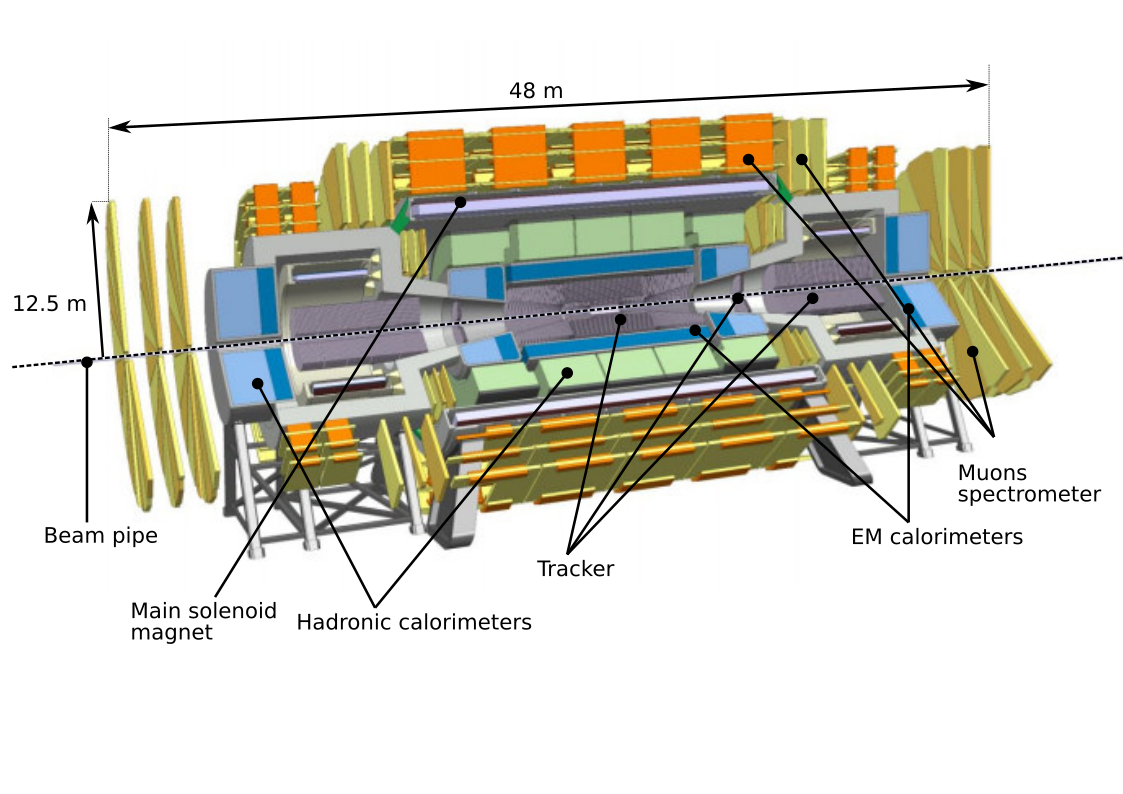
\includegraphics[trim={0 4cm 0.5cm 0},clip,width=\textwidth]{./Figures/FCCsvg1.png}
	\caption{FCC detector baseline concept.}
	\label{fig:FCC_detector}
\end{figure} 

%\begin{figure}
%	\centering
%	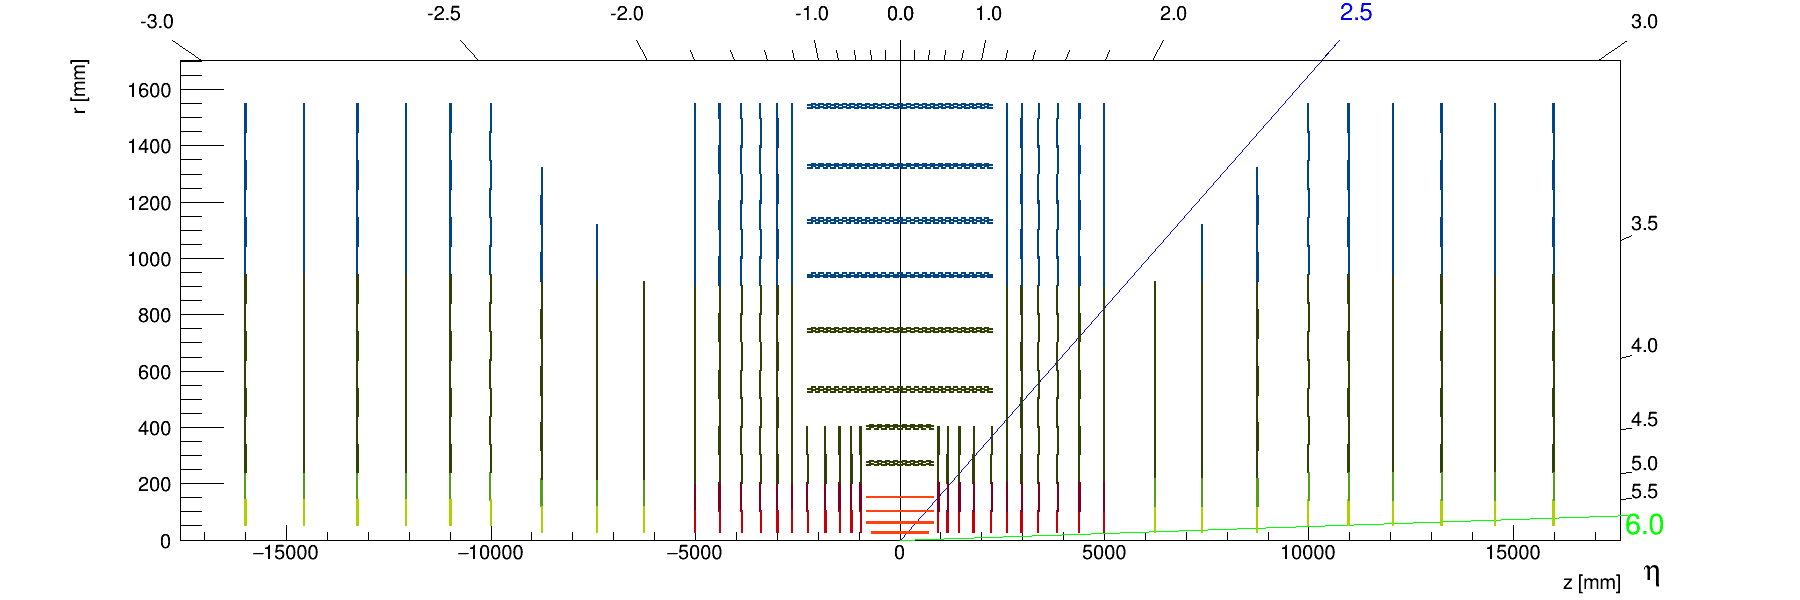
\includegraphics[trim={2cm 0 2cm 0},clip,width=\textwidth]{./Figures/FCC_tracker.png}
%	\caption{FCC detector proposed tracker layout.}
%	\label{fig:FCC_tracker}
%\end{figure} 

\subsection{FCC-hh physics program}

The FCC-hh physics program is vast and diverse. Within the SM, it includes the study of gauge bosons pair production and heavy flavor production, the measurement of the top quark's properties and the the study of the EWSB mechanism via multi-Higgs production. In addition, heavy ions collisions will allow for a deeper understanding of the Quark-Gluon Plasma. From a BSM standpoint, searches for supersymmetric and dark matter particles in new kinematic regimes can be pursued. A comprehensive review of the physics potential of the FCC-hh can be found here \cite{FCCyellow}. This document collects the results of the many studies that have been carried out since the beginning of the FCC initiative, in 2014.

Regarding Higgs pair production, a maximum precision on the SM cross section of $3\%$ is expected to be achieve using the $b\overline{b}\gamma\gamma$ final state. This would allow to constraint the Higgs triple coupling to be $\lambda_{hhh}\in [0.97,1.03]$. The $hh\rightarrow b\overline{b}b\overline{b}$ would allow for a $5\%$ precision on the SM cross section and to constraint the triple coupling to be $\lambda_{hhh}\in [0.9,1.5]$. In spite of the larger background yield, the $b\overline{b}b\overline{b}$ channel provides a reasonable number of events in the tail of the $m_{hh}$ distribution. As discussed in section \ref{section:Higgs_pair}, the tail of this distribution does not have a large contribution from the triangle diagram. Therefore, the sensitivity to the Higgs triple coupling is expected to be smaller. However, the high energy regime can be more sensitive to new physics contributions which makes the $b\overline{b}b\overline{b}$ channel a very interesting one. 

The Higgs quartic coupling could be probed through triple Higgs production. In this case the most promising final state seems to be $b\overline{b}b\overline{b}\gamma\gamma$. This channel could constraint the Higgs quartic coupling to be $\lambda_{hhhh}\in [-4,16]$.